Again, we follow \cite{Bojak:2000eu}.
\begin{figure}[ht!]
	\begin{subfigure}[t]{.4\textwidth}
		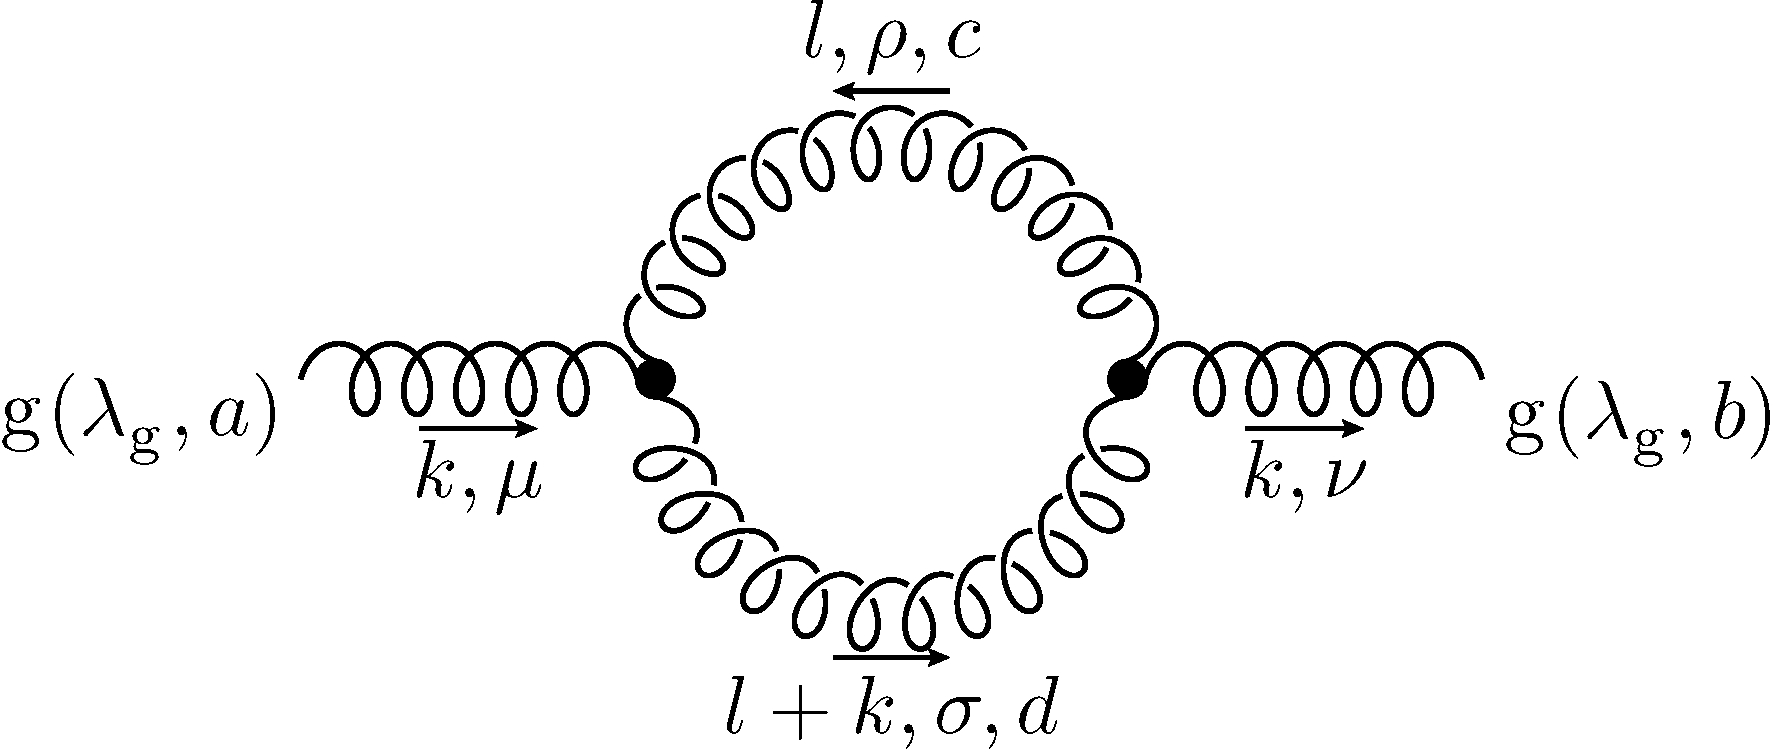
\includegraphics[width=\textwidth]{pyfeyn/nlo-v-seg}
		\caption{$-i\Pi_{\mu\nu}^{ab,(1)}(k)$}
	\end{subfigure}\hspace{.15\textwidth}%
	\begin{subfigure}[t]{.4\textwidth}
		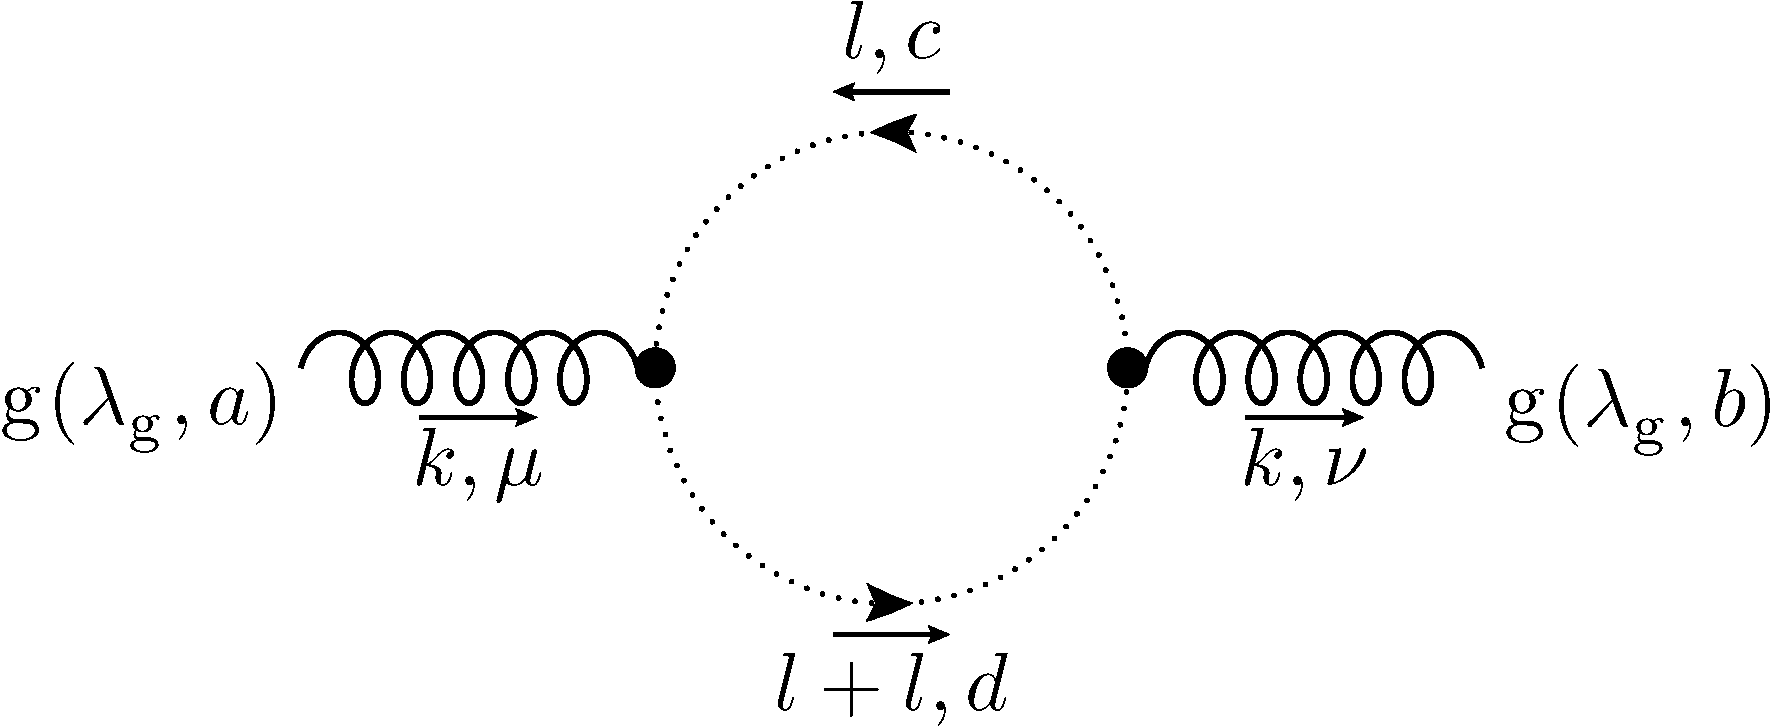
\includegraphics[width=\textwidth]{pyfeyn/nlo-v-seggh}
		\caption{$-i\Pi_{\mu\nu}^{ab,(2)}(k)$}
	\end{subfigure}\\
	\begin{subfigure}[t]{.4\textwidth}
		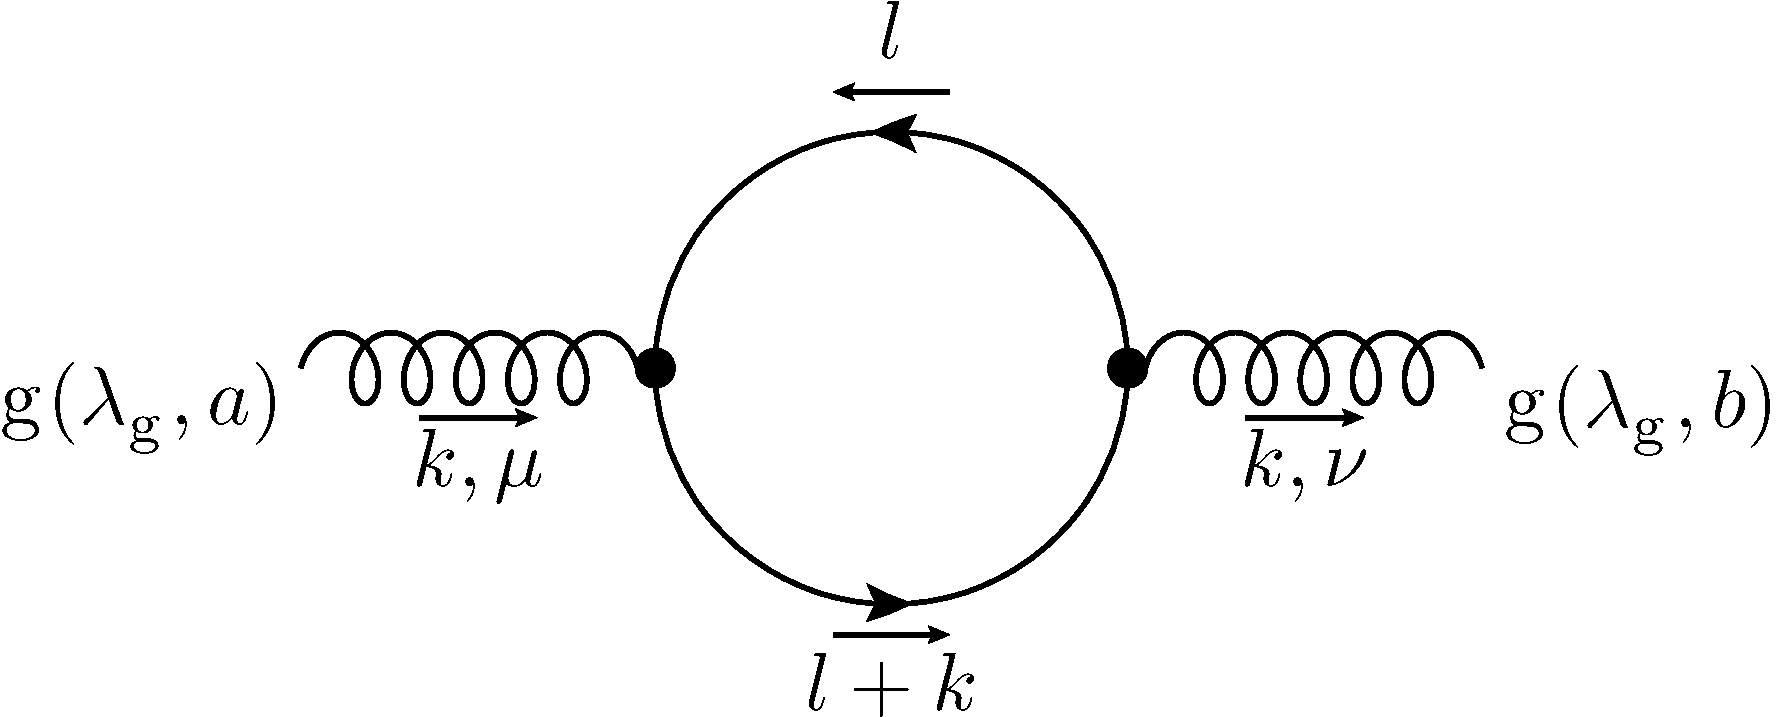
\includegraphics[width=\textwidth]{pyfeyn/nlo-v-segq}
		\caption{$-i\Pi_{\mu\nu}^{ab,(3)}(k)$}
	\end{subfigure}\hspace{.15\textwidth}%
	\begin{subfigure}[t]{.4\textwidth}
		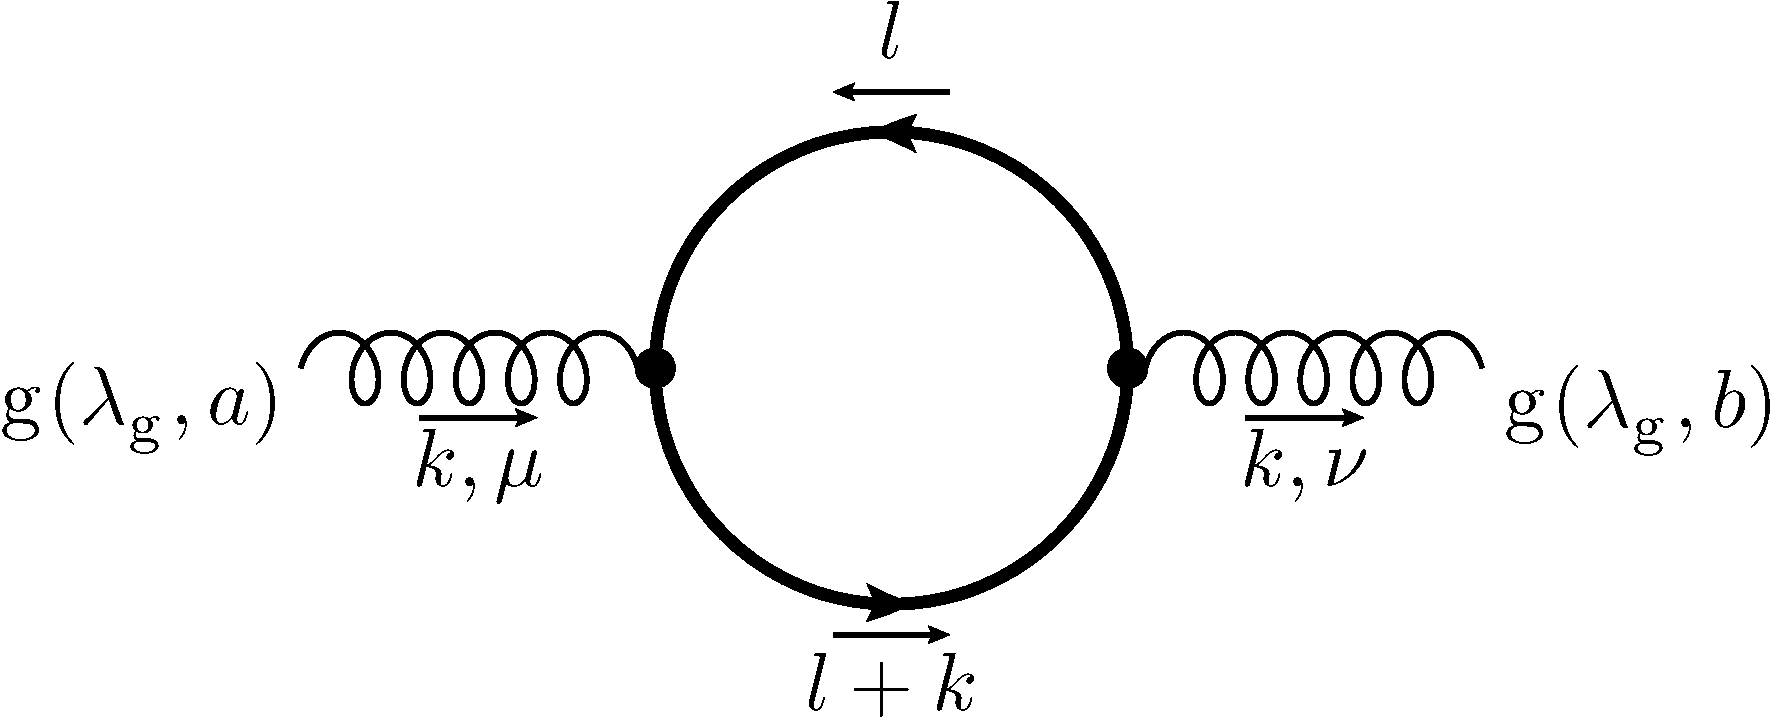
\includegraphics[width=\textwidth]{pyfeyn/nlo-v-seghq}
		\caption{$-i\Pi_{\mu\nu}^{ab,(4)}(k)$}
	\end{subfigure}\\
	\begin{subfigure}[t]{.4\textwidth}
		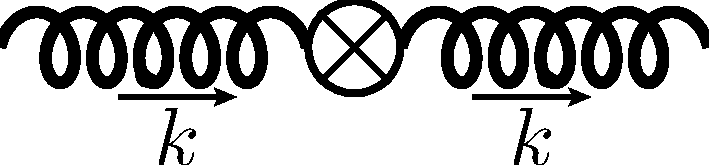
\includegraphics[width=\textwidth]{pyfeyn/nlo-v-segc}
		\caption{$-i\Pi_{\mu\nu}^{ab,(C)}(k)$}
	\end{subfigure}
	\caption{NLO contributions by quark self energy}\label{fig:FeynNLOvseqg}
\end{figure}

\begin{align}
-i\Pi_{\mu\nu}^{ab,(1)}(k) &= \frac 1 {2!} \mu_R^{4-n}\!\!\int\!\!\frac{d^nl}{(2\pi)^n} gf_{cda}\left(g_{\rho\sigma}(2l+k)_{\mu}+g_{\sigma\mu}(-l-2k)_\rho+g_{\mu\rho}(k-l)_\sigma\right)\nonumber\\
 &\hspace{30pt}\cdot gf_{cbd}\left(g^\rho_{\ \nu}(k-l)^\sigma+g_{\ \nu}^\sigma(-l-2k)^\rho+g^{\sigma\rho}(2l+k)_\nu\right)\cdot\frac{(-i)^2}{l^2(l+k)^2}\\
-i\Pi_{\mu\nu}^{ab,(2)}(k) &= -\mu_R^{4-n}\!\!\int\!\!\frac{d^nl}{(2\pi)^n} g^2 f_{adc}f_{bcd}l_\mu(l+k)_{\nu}\frac{i^2}{l^2(l+k)^2}\\
-i\Pi_{\mu\nu}^{ab,(3)}(k) &= -\mu_R^{4-n}\!\!\int\!\!\frac{d^nl}{(2\pi)^n} \frac{\tr\!\left((ig\gamma_\mu)(i\slashed l)\left(ig\gamma_\nu\right)(i(\slashed l + \slashed k))\right)\tr(T_aT_b)}{l^2(l+k)^2}\\
-i\Pi_{\mu\nu}^{ab,(4)}(k) &= -\mu_R^{4-n}\!\!\int\!\!\frac{d^nl}{(2\pi)^n} \frac{\tr\!\left((ig\gamma_\mu)(i(\slashed l + m))\left(ig\gamma_\nu\right)(i(\slashed l + \slashed k + m))\right)\tr(T_aT_b)}{(l^2-m^2)((l+k)^2-m^2)}\\
-i\Pi_{\mu\nu}^{ab,(C)}(k) &= i(Z_3-1)\delta^{ab}(k_\mu k_\nu-k^2g_{\mu\nu})
\end{align}

Color space:
\begin{align}
f_{acd}f_{bdc} &= -\delta_{ab} C_A = f_{dca}f_{dbc}\\
\tr(T_aT_b) &= \frac 1 2 \delta_{ab}
\end{align}

By Slavnov-Taylor\fxerror{cite} we know:
\begin{align}
\Pi_{\mu\nu}^{ab}(k) &= \delta^{ab}(k_\mu k_\nu-k^2g_{\mu\nu})\Pi(k^2)\\
\Rightarrow \Pi(k^2) &= -\frac{\delta_{ab}}{N_c^2-1}\frac 1 {(3+\epsilon)k^2}g^{\mu\nu}\Pi_{\mu\nu}^{ab}(k)
\end{align}

Gluon + Ghost loop:
\begin{align}
\Pi^{(1+2)}(k^2) &= -ig^2C_A\frac {1} {(3+\epsilon)k^2}\mu_R^{-\epsilon}\!\!\int\!\!\frac{d^nl}{(2\pi)^n} \frac{(8+3\epsilon)k\cdot l+(9+3\epsilon)k^2+(8+3\epsilon)l^2}{l^2(l+k)^2}\\
&= -ig^2C_A\frac {10+3\epsilon} {2(3+\epsilon)}\mu_R^{-\epsilon}\!\!\int\!\!\frac{d^nl}{(2\pi)^n} \frac{1}{l^2(l+k)^2}
\end{align}
with
\begin{align}
B_0(k^2,0,0) &= \mu_R^{-\epsilon}\!\!\int\!\!\frac{d^nl}{(2\pi)^n} \frac{1}{l^2(l+k)^2}\\
 &=\frac{i}{16\pi^2}\left(-\frac 2 {\hat\epsilon} -\ln(-k^2/\mu_R^2) + 2\right)
\end{align}
We find
\begin{align}
\Rightarrow \Pi^{(1+2)}(k^2) &= g^2C_A\left(-\frac {10} {3\hat\epsilon} - \frac 5 3\ln(-k^2/\mu_R^2) +\frac{31}{9}\right)\\
 &=-C_A\frac{g^2}{16\pi^2}\frac{5}{3}\left(\frac {2} {\hat\epsilon} + \ln(-k^2/\mu_R^2) -\frac{31}{15}\right)
\end{align}

Heavy quark loop:
\begin{align}
\Pi^{(4)}(k^2) &= ig^2\frac {1} {2(3+\epsilon)k^2}\mu_R^{-\epsilon}\!\!\int\!\!\frac{d^nl}{(2\pi)^n} \frac{4((2+\epsilon)(m^2-k\cdot l - l^2)+2m^2)}{(l^2-m^2)((l+k)^2-m^2)}\\
 &= ig^2\frac {2}{(3+\epsilon)k^2}\left(2m^2B_0(k^2,m^2,m^2)-(2+\epsilon)A_0(m^2)\right.\nonumber\\
 &\hspace{60pt}\left.-(2+\epsilon)k^2B_1(k^2,m^2,m^2)\right)
\end{align}
with
\begin{align}
A_0(m^2) &= \frac {i m^2}{16\pi^2}\left(-\frac 2 {\hat \epsilon_m} + 1 \right)\\
B_1(k^2,m^2,m^2) &= -\frac 1 2 B_0(k^2,m^2,m^2)\\
B_0(k^2,m^2,m^2) &= \frac i {16\pi^2}\left(-\frac 2 {\hat \epsilon_m} + 2 + \beta_k\ln(\chi_k) \right)
\end{align}
and $\beta_k=\sqrt{1-4m^2/k^2}$, $\chi_k=(\beta_k-1)/(1+\beta_k)$. We then find
\begin{align}
\Rightarrow \Pi^{(4)}(k^2) &= \frac {2g^2}{16\pi^2}\left(\frac 2 {3\hat \epsilon_m}-\frac 5 9 -\frac{4m^2}{3k^2} - \frac 1 3 \left(1+2\frac{m^2}{k^2}\right)\beta_k\ln(\chi_k)\right)\\
&= \frac {g^2}{16\pi^2}\frac 2 3\left(\frac 2 {\hat \epsilon_m}-\frac 5 3 -4\frac{m^2}{k^2} - \left(1+2\frac{m^2}{k^2}\right)\beta_k\ln(\chi_k)\right)
\end{align}

Light quark loop:
\begin{align}
\Pi^{(3)}(k^2) &= -ig^2\frac {2(2+\epsilon)}{(3+\epsilon)}B_1(k^2,0,0)\\
 &= ig^2\frac {(2+\epsilon)}{(3+\epsilon)}B_0(k^2,0,0)\\
 &=\frac{g^2}{16\pi^2}\frac 2 3\left(\frac 2 {\hat \epsilon} + \ln(-k^2/\mu_R^2)-\frac 5 3\right)
\end{align}

We choose the counterterm to be:
\begin{align}
-\Pi^{(C)}(k^2)=Z_3-1 &= \frac{g^2}{16\pi^2}\left(-\frac 5 3 C_A \frac 2 {\hat \epsilon} + n_{lf}\frac 2 3 \frac 2 {\hat \epsilon} + \frac 2 3 \frac 2 {\hat \epsilon_m}\right)\\
 &= \frac{g^2}{16\pi^2}\left( (2C_A-\beta_0)\frac 2 {\hat\epsilon}+ \frac 2 3 \frac 2 {\hat \epsilon_m} \right)\\
 &= \frac{g^2}{16\pi^2}\left( (2C_A-\beta_0^f)\frac 2 {\hat\epsilon}+ \frac 2 3 \ln(m^2/\mu^2) \right)
\end{align}
with $\beta_0 = (11C_A-2n_{lf})/3$ and $\beta_0^f = (11C_A-2n_{f})/3$.
